% \documentclass[dvipdfmx, 11pt]{beamer}
\documentclass[aspectratio=43, dvipdfmx, 11pt]{beamer} % aspectratio=43, 149, 169
\usepackage{here, amsmath, latexsym, amssymb, bm, ascmac, mathtools, multicol, tcolorbox, subfig}
\usepackage{float}
\usepackage{newtxtext,newtxmath}
\usepackage{algpseudocode}
\usepackage{braket}
\usepackage{fancybox}
%\usepackage{algorithm, algpseudocode}

%デザインの選択(省略可)
\usetheme{Luebeck}
%カラーテーマの選択(省略可)
\usecolortheme{orchid}
%フォントテーマの選択(省略可)
\usefonttheme{professionalfonts}
%フレーム内のテーマの選択(省略可)
\useinnertheme{circles}
%フレーム外側のテーマの選択(省略可)
\useoutertheme{infolines}
%しおりの文字化け解消
\usepackage{atbegshi}
\ifnum 42146=\euc"A4A2
\AtBeginShipoutFirst{\special{pdf:tounicode EUC-UCS2}}
\else
\AtBeginShipoutFirst{\special{pdf:tounicode 90ms-RKSJ-UCS2}}
\fi
%ナビゲーションバー非表示
\setbeamertemplate{navigation symbols}{}
%既定をゴシック体に
\renewcommand{\kanjifamilydefault}{\gtdefault}
%タイトル色
\setbeamercolor{title}{fg=structure, bg=}
%フレームタイトル色
\setbeamercolor{frametitle}{fg=structure, bg=}
%スライド番号のみ表示
%\setbeamertemplate{footline}[frame number]
%itemize
\setbeamertemplate{itemize item}{\small\raise0.5pt\hbox{$\bullet$}}
\setbeamertemplate{itemize subitem}{\tiny\raise1.5pt\hbox{$\blacktriangleright$}}
\setbeamertemplate{itemize subsubitem}{\tiny\raise1.5pt\hbox{$\bigstar$}}
% color
\newcommand{\red}[1]{\textcolor{red}{#1}}
\newcommand{\green}[1]{\textcolor{green!40!black}{#1}}
\newcommand{\blue}[1]{\textcolor{blue!80!black}{#1}}

\newcommand{\argmax}{\mathop{\rm arg~max}\limits}

\title[BPR]{BPR$\colon$Bayesian Personalized Ranking}
\subtitle{}
\author[山田倫太郎]{Steffen Rendle, Christoph Freudenthaler, Zeno Gantner, Lars Schmidt-Thieme}
\institute[竹内・烏山研究室]{Presenter: 山田倫太郎}
\date{\today}

\begin{document}
\maketitle

\begin{frame}{研究背景}
    推薦システムにおいて個人の嗜好を予測することは重要\\
    \vspace{6mm}
    大別すると2種類のデータが考えられる
    \begin{itemize}
        \item Explicit feedback
            \begin{itemize}
                \item ユーザの興味が明示的に与えられているデータ\\
                \quad 例) Amazonの☆やfacebookの「いいね」
            \end{itemize}
        \item \alert{Implicit feedback}
            \begin{itemize}
                \item ユーザの興味が明示的に与えられてないデータ\\
                \quad 例) 購入履歴や閲覧履歴
            \end{itemize}
    \end{itemize}
        \begin{block}{目標}
        Implicit feedbackを元にユーザの嗜好をランキングする
        \end{block}{}
\end{frame}

\begin{frame}{従来法}

    閲覧されたか否かを{0,1}のラベルで表現
    \begin{tabular}{ll}
        \begin{minipage}{0.4\hsize}
        \begin{flushleft}
        \begin{equation*}
        \begin{aligned}
            u \colon & \, \text{ユーザ}\\
            i \colon & \, \text{アイテム}\\
            + \colon & \, \text{閲覧済み}\\
            ? \colon & \, \text{未閲覧}\\
        \end{aligned}
        \end{equation*}
    \end{flushleft}
    \end{minipage}
    \begin{minipage}{0.6\hsize}
        \begin{figure}[H]
        \begin{flushleft}
        \vspace{1zh}
        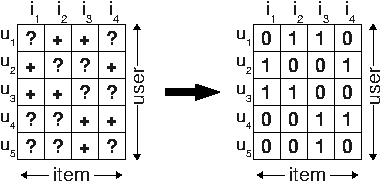
\includegraphics[pagebox=cropbox,clip]{BPR-crop.pdf}
        %\vspace*{-0.5cm} % 図とキャプションの間隔
        %\caption{1 番目の図}
        %\label{Figure: 1 番目の図}
    \end{flushleft}
        \end{figure}
    \end{minipage}
    \end{tabular}
    \begin{alertblock}{問題点}
    未閲覧のデータ中で以下を区別できない
        \begin{itemize}
            \item ユーザの興味がないもの
            \item ユーザの興味があるが閲覧していないもの
        \end{itemize}
    \end{alertblock}
\end{frame}

\begin{frame}{提案手法}
    \begin{block}{方針}
        ユーザの選好関係をモデル化する\\
    \end{block}

    仮定$\colon$ 閲覧済みアイテムの興味 > 未閲覧アイテムの興味
        \begin{figure}[H]
        \begin{center}
        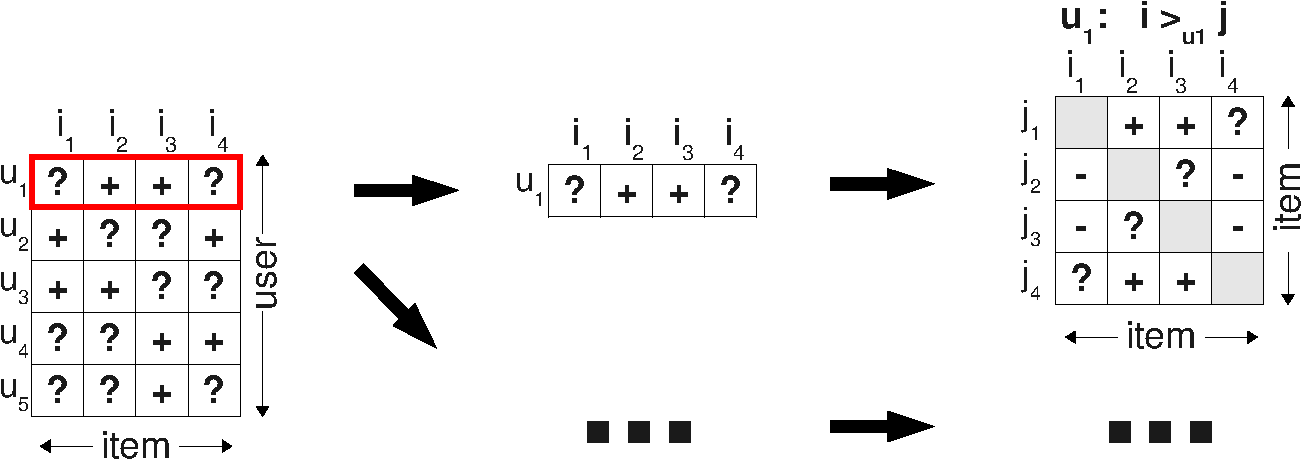
\includegraphics[scale=0.55,pagebox=cropbox,clip]{new-crop.pdf}
        \end{center}
        \end{figure}
\end{frame}

\begin{frame}{記法}
    \begin{itemize}
    \item $U \colon \text{ユーザの全体集合}$\\
    \item $I \colon \text{アイテムの全体集合}$\\
    \item $U^+_i \colon \text{アイテムiを閲覧したユーザの全体集合}$\\
    \item $I^+_u \colon \text{ユーザuが閲覧したアイテムの全体集合}$\\
    \item $D_s \colon \text{フィードバックが得られているデータセット}$\\
    \begin{itemize}
        \item $D_s \coloneqq \{(u,i,j) \mid i \in I^+_u \land j \in I\backslash I^+_u \}$
    \end{itemize}
    \item $>_u \colon \text{ユーザ}u\text{の嗜好情報}$\\
    \item $\Theta \colon \text{モデルパラメータ}$\\
    \item $x_{ui} \colon \text{ユーザ}u\text{のアイテム}i\text{の選好度合い}$
    \end{itemize}

$x_{ui}$は推論モデルによって既定される値なのでパラメータ$\Theta$に依存\\
\vspace{5mm}
$D_s$よりパラメータ$\Theta$を導出したいので $p(\Theta \mid D_s)$を最適化
\end{frame}

\begin{frame}{モデリング}
    ベイズの定理より次の式が導かれる$\colon$
    \[p(\Theta \mid D_s) \propto p(D_s \mid \Theta) p(\Theta)\]
                
    ユーザ, アイテムの好みが独立であると仮定し,尤度を以下で定める$\colon$ 

    \[\prod_{(u,i,j)\in D_s} p(i >_u j \mid \Theta)\]

    ここでシグモイド関数を$\sigma$として $\colon$

    \[p(i >_u j \mid \Theta) \coloneqq \sigma(\hat{x}_{ui}-\hat{x}_{uj})\]
\end{frame}

\begin{frame}{目的関数: BPR-Opt}
    \begin{itemize}
        \item 事前分布$p(\Theta)$は正規分布$N(0,\lambda_{\Theta}I)$とする 
        \item MAP推定を行う
    \end{itemize}
    \begin{equation*}
        \large{
    \begin{aligned}
        \hat{\Theta} &= \argmax_{\Theta} \; \ln{p(\Theta \mid D_s)}\\
                    &= \argmax_{\Theta} \; \ln{p(D_s \mid \Theta)p(\Theta)}\\
                    &= \argmax_{\Theta} \; \ln{\prod_{(u,i,j)\in D_s}\sigma(\hat{x}_{ui}-\hat{x}_{uj})p(\Theta)}
    \end{aligned}
        }
    \end{equation*}
    \begin{itemize}
        \item 以下の目的関数を最大化する
    \end{itemize}
    
    \Large \[\text{BPR-Opt} \coloneqq \sum_{(u,i,j) \in D_s} \ln \sigma(\hat{x}_{ui}-\hat{x}_{uj})-\frac{1}{2\lambda_{\Theta}}\|\Theta\|^2\]
\end{frame}

\begin{frame}{目的関数: BPR-Opt}
    
    \begin{itemize}
        \item BPR-Optを微分すると
    \begin{equation*}
        \Large{
    \begin{aligned}
        \frac{\partial \text{BPR-Opt}}{\partial \Theta} &= \sum_{(u,i,j) \in D_s} \frac{\partial}{\partial \Theta} \ln \sigma(\hat{x}_{ui}-\hat{x}_{uj})-\frac{1}{2\lambda_{\Theta}} \frac{\partial}{\partial \Theta} \|\Theta\|^2 \\
                                                 &= \frac{-e^{\hat{x}_{ui}-\hat{x}_{uj}}}{1+e^{\hat{x}_{ui}-\hat{x}_{uj}}} \cdot \frac{\partial}{\partial \Theta}(\hat{x}_{ui}-\hat{x}_{uj})-\frac{\Theta}{\lambda_{\Theta}}
    \end{aligned}
    }
\end{equation*}

   \item $(u,i,j) \in D_s$は膨大となりやすいので確率的勾配法を用いて解く
\end{itemize}
\end{frame}

\begin{frame}{学習アルゴリズム: Learn-BPR}
    \Large \begin{algorithmic}[1]
     \Procedure{Learn-BPR}{$D_s,\Theta$}
        \State initialize $\Theta$
        \Repeat
            \State draw (u,i,j) from $D_s$
            \State $\Theta \longleftarrow \Theta+\alpha(\frac{-e^{\hat{x}_{ui}-\hat{x}_{uj}}}{1+e^{\hat{x}_{ui}-\hat{x}_{uj}}} \cdot \alert{\frac{\partial}{\partial \Theta}(\hat{x}_{ui}-\hat{x}_{uj})}-\frac{\Theta}{\lambda_{\Theta}})$
        \Until{convergence}
        \State \textbf{return} $\hat{\Theta}$
        \EndProcedure
   \end{algorithmic}

   \begin{itemize}
   \item \Large $\frac{\partial}{\partial \Theta}(\hat{x}_{ui}-\hat{x}_{uj})$については次に示す
   \end{itemize}
\end{frame}
\begin{frame}{$x_{ui}$の具体例1 : Matrix Facterization}

    次元削減を行って$\hat{x}_{ui}$を推定する

    \begin{tabular}{ll}
    \begin{minipage}{0.7\hsize}
        \begin{flushleft}
    \begin{figure}[H]
        \vspace{1zh}
        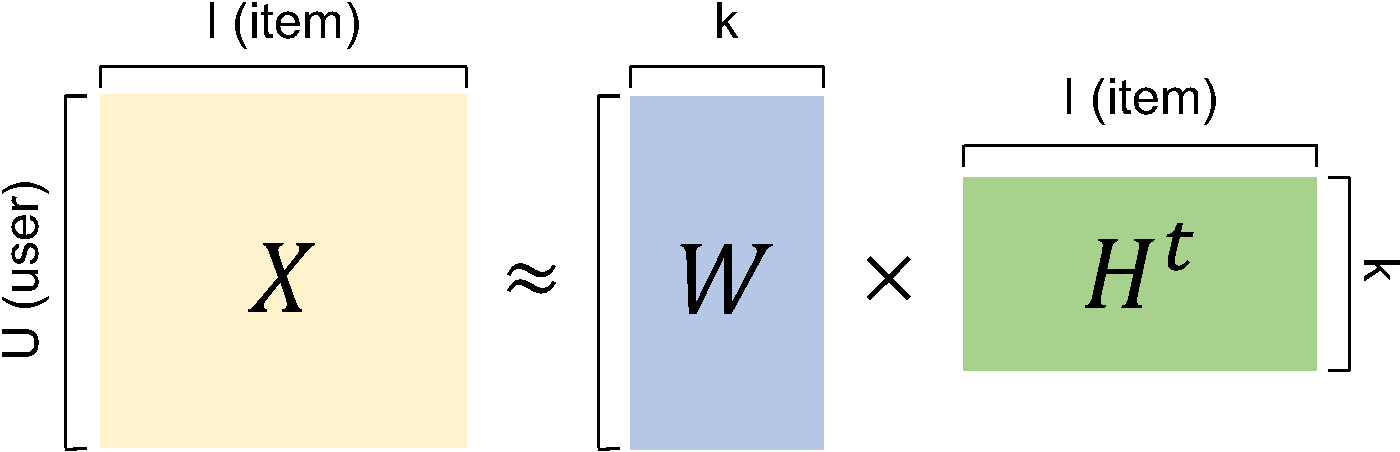
\includegraphics[scale=0.35,pagebox=cropbox,clip]{MF-crop.pdf}
        %\vspace*{-0.5cm} % 図とキャプションの間隔
        %\caption{1 番目の図}
        %\label{Figure: 1 番目の図}
    \end{figure}
\end{flushleft}
\end{minipage}
\begin{minipage}{0.3\hsize}
    \begin{center}
        \doublebox{
    $\hat{X} \coloneqq WH^T$
        }
    \end{center}
\end{minipage}
\end{tabular}

\begin{tabular}{ll}
   \begin{minipage}{0.3\hsize}
        \begin{flushleft}
        \begin{equation*}
            \begin{aligned}
                \hat{x}_{ui} &= \braket{w_u,h_i}\\
                            &= \sum_{f=1}^k w_{uf}\cdot h_{if}                    
            \end{aligned}
        \end{equation*}
         \end{flushleft}
    \end{minipage}
    \begin{minipage}{0.7\hsize}
        \begin{flushleft}
            \begin{equation*}
                \frac{\partial}{\partial \Theta}(\hat{x}_{ui}-\hat{x}_{uj})=
                \left\{
                \begin{aligned}
                &(h_{if}-h_{jf})\quad &\text{if}\ \theta&=w_{uf}\\
                &w_{uf}&\text{if}\ \theta&=h_{if}\\
                &-w_{uf}&\text{if}\ \theta&=h_{jf}\\
                &0 &\text{else}                \end{aligned}
                \right.
            \end{equation*}
        \end{flushleft}
    \end{minipage}
\end{tabular}{ll}
\end{frame}

\begin{frame}{$x_{ui}$の具体例2 : Adaptive k Nearest Neighbor}
    
    観測済みアイテムとの類似度をもとに$\hat{x}_{ui}$を推定する
    \LARGE \[\hat{x}_{ui}=\sum_{i \in I^+_u \land l \neq i}c_{il}\]

    \large    \begin{equation*}
            \begin{aligned}
                \frac{\partial}{\partial \Theta}(\hat{x}_{ui}-\hat{x}_{uj})=
                \left\{
                \begin{aligned}
                &+1 \quad &\text{if}\ \theta&\in \{c_{il},c_{li}\} \land l\in I^+_u \land l \neq i\\
                &-1&\text{if}\ \theta&\in \{c_{jl},c_{lj}\} \land l\in I^+_u \land l \neq j\\
                &0 &\text{else}
            \end{aligned}
                \right.
    \end{aligned}
            \end{equation*}
    

\end{frame}

\begin{frame}{実験}
    \begin{enumerate}
        \item Rossmannオンラインショップの購入履歴から, ユーザが次に買いたい品物を予測
        \item Netflixの過去の映画の評価履歴をもとに, 与えられた映画に評価を行うかを予測
    \end{enumerate}
    \begin{table}[htb]
        \begin{tabular}{|c|c|c|c|} \hline
                    &ユーザー(人)&アイテム(個) &観測済み(個) \\ \hline
        Rossmann    &10,000       &4,000       &436,612 \\\hline
        Netflix     &10,000       &5,000       &565,738 \\ \hline
        \end{tabular}
      \end{table}
      \begin{itemize}
        \item ROC曲線のAUCを評価
      \end{itemize}
\end{frame}

\begin{frame}{比較手法}
    \begin{itemize}
        \item \alert{BPR-MF}
        \begin{itemize}
            \item パラメータの更新にBPR-Optを用いたMF
        \end{itemize}
        \item \alert{BPR-kNN}
        \begin{itemize}
            \item パラメータの更新にBPR-Optを用いたk近傍
        \end{itemize}
        \item SVD-MF 
        \begin{itemize}
            \item SVD(特異値分解)を適応したもの
        \end{itemize}
        \item WR-MF
        \begin{itemize}
            \item SVD(特異値分解)の過学習を抑えるように改良したもの
        \end{itemize}
        \item Cosine-kNN
        \begin{itemize}
            \item コサイン類似度を用いたk近傍法
        \end{itemize}
        \item most popular
        \begin{itemize}
            \item 学習データの中で最も人気のものを推薦する
        \end{itemize}
        \item $\text{np}_{\text{max}}$
        \begin{itemize}
            \item テストデータの中で最も人気のものを推薦する
        \end{itemize}
    \end{itemize}
\end{frame}

\begin{frame}{結果}
    \begin{figure}[H]
        \begin{tabular}{cc}
        \begin{minipage}{0.5\hsize}
            \begin{flushleft}
          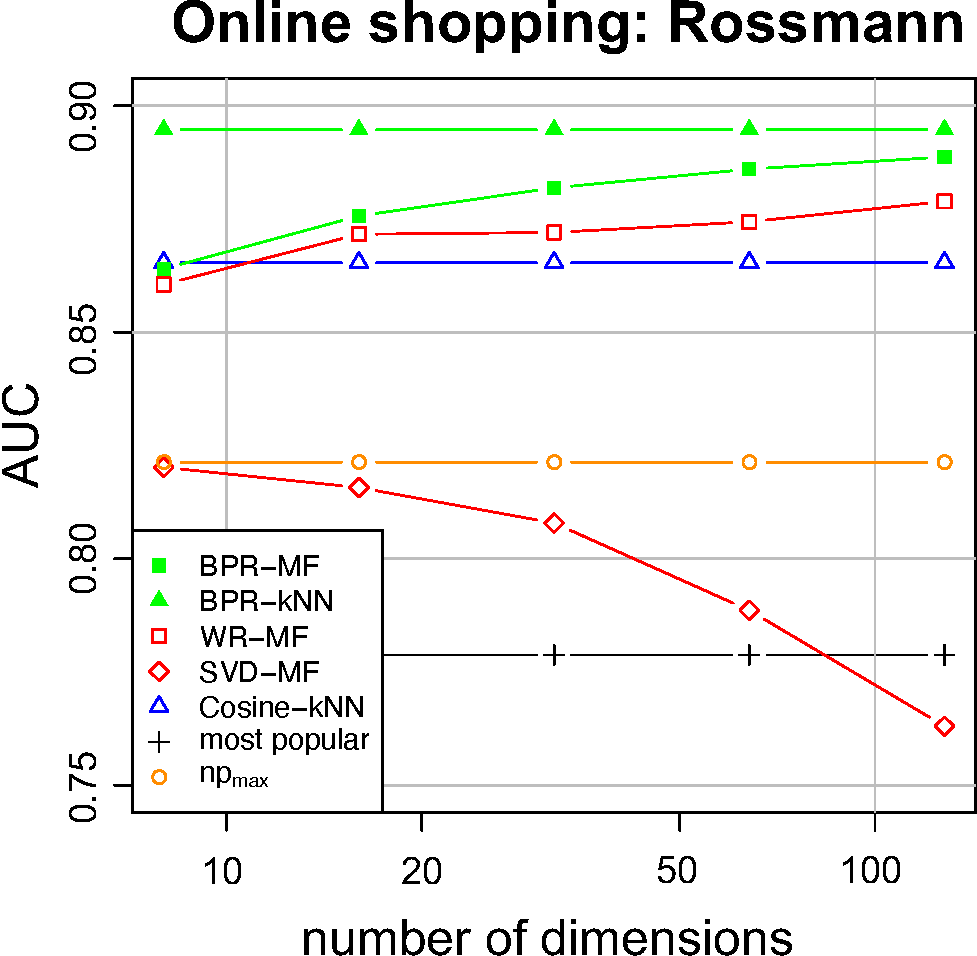
\includegraphics[scale=0.35]{ross-crop.pdf}
            \end{flushleft}
        \end{minipage}
        \begin{minipage}{0.5\hsize}
            \begin{flushleft}
          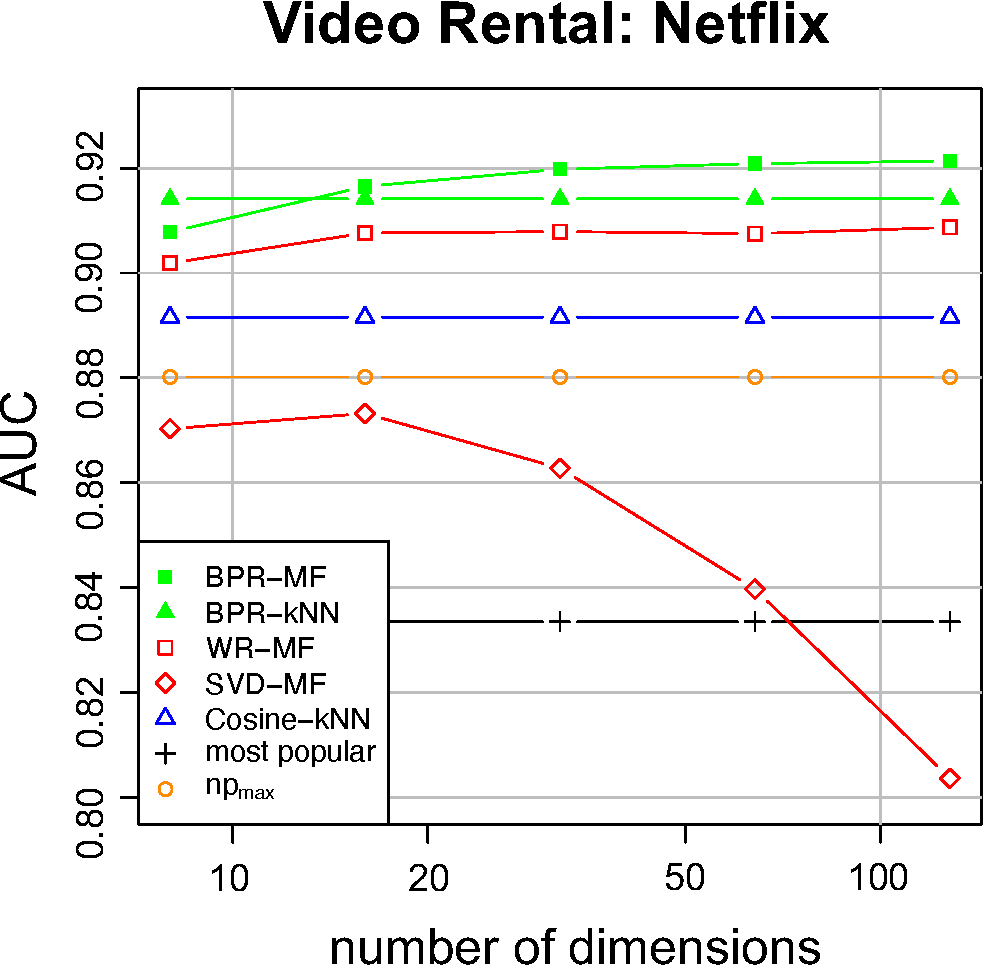
\includegraphics[scale=0.35]{net-crop.pdf}
            \end{flushleft}
        \end{minipage}
    \end{tabular}
    \end{figure}
    
    実験において提案手法が他のモデルよりも優れた結果を示した
\end{frame}

\begin{frame}{まとめ}
    \begin{block}{BPRの手法}
        \begin{itemize}
            \item 閲覧済みアイテムは未閲覧アイテムより興味があると仮定を置く
            \item ユーザのアイテム同士の選好関係をモデル化する
            \item パラメータ最適化に確率的勾配法を用いる
        \end{itemize}
    \end{block}

    \begin{block}{結果}
        BPRによるパラメータ最適化が他のモデルよりも優れている
    \end{block}

\end{frame}

\end{document}